\documentclass[9pt]{memoir}

\usepackage[osf]{mathpazo}
\usepackage[mathcal,mathbf]{euler}
\usepackage{amsmath,amssymb,amsthm}
\usepackage[utf8]{inputenc}
\usepackage{graphicx,sidecap,tikz}
\usepackage{siunitx} % automatic number formatting, decimal point alignment
\usepackage[breaklinks=true]{hyperref} % automatic links to sections, figures, http, etc...
\usepackage{textcomp} % needed to the \bullet symbol on lists

% BibTex references
\usepackage[]{natbib}
\usepackage{aas_macros} % Astronomical Journals abreviations
\bibliographystyle{astron} % Astronomy bibliography style

% To get lining figures in tables set by siunitx, which apparently uses the
% \mathrm font instead of \mathnormal
\SetMathAlphabet{\mathrm}{normal}{U}{eur}{m}{n}

%%% William Defs %%% 


% =========================
% = Setting up the layout =
% =========================

% With a 9pt body font we want a little extra line spacing (I mean *leading*)
\setSingleSpace{1.2}
\SingleSpacing

% Okay, holy crap. Calculating the correct type block height by hand is quite
% challenging (partially because not all lines are \baselineskip high;
% apparently the first line is \topskip high?), and \checkandfixthelayout will
% in the end actually *change* it so that the type block is always an integer
% multiple of lines. The easiest thing is to set the approximate desired type
% block height, the width, the left or right margin, the bottom margin, and
% the headdrop, and then let memoir take care of everything else. Changing the
% algorithm used to check the layout helps as well.
\setstocksize{9in}{6in}
\settrimmedsize{\stockheight}{\stockwidth}{*}
\settrims{0pt}{0pt}

\settypeblocksize{46\baselineskip}{4in}{*}
\setlrmargins{*}{0.5in}{*}
\setulmargins{*}{0.5in}{*}

\setheadfoot{\baselineskip}{\baselineskip} % headheight and footskip
\setheaderspaces{0.5in}{*}{*} % headdrop, headsep, and ratio

\checkandfixthelayout[lines]

% Set up custom headers and footers
\makepagestyle{stylish}
\copypagestyle{stylish}{headings}
\makerunningwidth{stylish}{5in}
\makeheadposition{stylish}{flushleft}{flushright}{}{}
\pagestyle{stylish}

% ============================
% = Table of contents tweaks =
% ============================
\renewcommand*{\contentsname}{Table of Contents}
\setsecnumdepth{subsubsection}
\settocdepth{subsection}

% ============
% = Chapters =
% ============
\newcommand{\swelledrule}{%
    \tikz \filldraw[scale=.015,very thin]%
    (0,0) -- (100,1) -- (200,1) -- (300,0) --%
    (200,-1) -- (100,-1) -- cycle;}
\makeatletter
\makechapterstyle{grady}{%
    \setlength{\beforechapskip}{0pt}
    \renewcommand*{\chapnamefont}{\large\centering\scshape}
    \renewcommand*{\chapnumfont}{\large}
    \renewcommand*{\printchapternum}{%
        \chapnumfont \ifanappendix \thechapter \else \numtoName{\c@chapter}\fi}
    \renewcommand*{\printchapternonum}{%
        \vphantom{\printchaptername}%
        \vphantom{\chapnumfont 1}%
        \afterchapternum
        \vskip -\onelineskip}
    \renewcommand*{\chaptitlefont}{\Huge\itshape}
    \renewcommand*{\printchaptertitle}[1]{%
        \centering\chaptitlefont ##1\par\swelledrule}}
\makeatother
\chapterstyle{grady}

% See below, after introduction, for \clearforchapter

% Prevent page numbers from appearing on chapter pages
\aliaspagestyle{chapter}{empty}

% ===================
% = Marginal labels =
% ===================
\strictpagecheck % Turn on robust page checking
\captiondelim{} % Don't print a colon after "Figure #.#"

\makeatletter
\renewcommand{\fnum@figure}{%
    \checkoddpage%
    \ifoddpage%
        \makebox[0pt][l]{\hspace{-1in}{\scshape\figurename~\thefigure}}%
    \else
        \makebox[0pt][r]{{\scshape\figurename~\thefigure}\hspace*{-5in}}%
    \fi%
    }
\renewcommand{\fnum@table}{%
    \checkoddpage%
    \ifoddpage%
        \makebox[0pt][l]{\hspace{-1in}{\scshape\tablename~\thetable}}%
    \else
        \makebox[0pt][r]{{\scshape\tablename~\thetable}\hspace*{-5in}}%
    \fi%
    }
\let\mytagform@=\tagform@
\def\tagform@#1{%
\checkoddpage%
    \ifoddpage%
    \makebox[1sp][l]{\hspace{-5in}\maketag@@@{(\ignorespaces#1 \unskip \@@italiccorr)}}%
    \else
    \makebox[1sp][r]{\maketag@@@{(\ignorespaces#1 \unskip \@@italiccorr)}\hspace*{-1in}}%
    \fi%
    }
\renewcommand{\eqref}[1]{\textup{\mytagform@{\ref{#1}}}}
\makeatother

\usetikzlibrary{arrows,positioning,decorations.pathmorphing,trees}

\begin{document}

\frontmatter
\thispagestyle{empty}

\begin{figure}
	\vspace{-10pt}
	\begin{adjustwidth*}{-1in}{0pt}
		\centering
		
\includegraphics[width=0.3\textwidth]{figures/Escudo_de_la_Universidad_de_Granada.pdf}
	\end{adjustwidth*}
	\vspace{-15pt}
\end{figure}


\begin{adjustwidth*}{-1in}{0pt}
	\centering
	\makebox[0pt]{\scshape{}Universidad de Granada} \par
	\makebox[0pt]{\scshape{}FisyMat} \par
\end{adjustwidth*}

\mbox{}\vspace{1.8in}
\noindent
\begin{flushright}
{\LARGE\itshape{}a}\hspace{1.5em}{\HUGE\scshape{}Book}\\[2\baselineskip]
{\LARGE\itshape{}of}\hspace{1.5em}{\Huge\scshape{}Fascinating Facts}
\end{flushright}

\vspace{6\baselineskip}
\hfill{\LARGE\scshape{}William Schoenell}

\vspace{1\baselineskip}
\hfill{\Large\scshape{}Advised by: Narciso Ben\'\i tez}


\cleartorecto\tableofcontents*

\mainmatter

\chapter{Introduction}
Say about the importance of measuring galaxies properties.

\section{Surveys}

\section{The A-PLUS survey}

\section{The J-PAS survey}

\chapter{The southern A-PLUS telescope}

In this chapter we describe the design and the installation of the Brazilian counterpart of the 86 cm telescope installed on Teruel. The T80S telescope is a \textbf{ improve this} founded project by the Brazilian institutions IAG, ON and LNA. The main objective for building the telescope is to carry two surveys the A-PLUS and the S-POL. The A-PLUS will be a photometric survey on the southern hemisphere \textbf{ meter figura da area} on twelve optical filters \textbf{ TODO meter tabela e curavs}. The S-POL (tbd).

\section{T80S installations}
The T80-South telescope is situated near the summit of Cerro Tololo in central Chile, at an altitude of 2,207 m, at latitude -30:10:10.78 and longitude -70:48:23.49. It is installed on a small building with the dome, a small data center for data processing and two auxiliary rooms for instrument engineering purposes. The operation of the telescope is designed to be fully automated and it is controlled by the observatory control system (OCS) developed by our team \textbf{explain better} since 2008. More details of the OCS will be described on \ref{sec:chimera}.

\subsection{Telescope}

The T80S is a new generation of Ritchey-Chretien Cassegrain telescopes with a huge field of view (FoV) of 2 square degrees. The design of telescopes with such FoVs are crucial to conduct astromical surveys as it allows to cover huge areas on the sky with relatively small amounts of time. The telescope design was developed by Advanced Mechanical and Optical Systems (AMOS) in Liège, Belgium with the mechanical fabrication, assembly and control systems subcontracted to the German company ASTELCO Systems GmbH in Munich. The telescope control is done via a private protocol called OpenTPL developed by Tau-Tec GmbH. More details on the control of the telescope are explained on section \ref{sec:chimera}.

The telescope detailed optical parameters are shown on table \ref{tab:t80s_optics}.

\begin{table}
\label{tab:t80s_optics}
\begin{tabular}{
    r
    S[table-format=1.3]
    S[table-format=3.5e-1]
    S[table-format=1.4]
    S[table-format=-1.5]
}
\toprule			
Primary Mirror (M1)	&		\\ \midrule
Curvature radius	&	{$-2471.295 mm$ concave}	\\
Conic constant	&	-1.163946	\\
Optical Diameter	&	{$826 mm$}	\\
Central hole	&	\textbf{TODO}	\\
Used clear aperture	&	\textbf{TODO}	\\
Effective collecting area	&	{$0.44 m^2$}	\\ \midrule
Secondary F/4.5 mirror (M2)	&		\\ \midrule
Distance from Primary	&	{$825.7695 mm$}	\\
Radius of curvature	&	{$-1237.411 mm$ convex}	\\
Conic constant	&	-5.776745	\\
Optical Diameter	&	{$302.879 mm$}	\\
\bottomrule					
\end{tabular}
\caption{T80S telescope optical specifications}
\end{table}

The alignment of the secondary mirror with respect of the primary mirror needs to be done on each pointing due the large FoV area. The telescope center of mass and temperature changes the alignment, so a simple model was implemented by 

\subsection{Instrument}

On both photometric and polarimetric mode, T80S will use a Spectral Instruments 1100S camera equipped with an E2V 290-99-1-F24 CCD (serial number 11323-24-01). This CCD is mounted on the focal plane with a filter+shutter unit (FSU) \textbf{ figure here!} between it and the telescope flange. The filter shutter unit is composed of a custom-made shutter by Bonn Shutters and filter wheels with their motors and encoders according the observation model (polarimetric or photometric).

The mechanical part of the FSU was designed at Instituto de Pesquisas Espaciais, in Brazil, and produced by MetalCard. The control of the FSU was designed by another Brazilian company Solunia using Programable Logic Controllers PLCs from Beckhoff.

On the photometric mode, the FSU counts with two filter wheels with 7 positions each (6 filters plus 1 clear position) and it also hosts a guiding camera at the border of the focal plane which is not used at the moment since the telescope tracking is sufficiently accurate for the exposure times of the survey \textbf{ cite table survey exposure times}.

\textbf{ TODO: EXPAND ON THIS On the polarimetric mode, the FSU counts with one filter wheel, one polarimetric wheel which spins a crystal of calcite, giving the required polarization phase for each exposure and one ???}

%\begin{figure}
%\begin{adjustwidth*}{-1in}{0pt}
%\centering
%\begin{tikzpicture}[domain=-0.62:10.85,decoration={random steps,segment length=1pt,amplitude=0.3pt}]
%    \draw[very thin,color=gray,decorate] (-1.25,-1.25) grid (11.25,1.25);
%    \draw[color=orange,decorate] plot (\x,{sin(\x r)});
%\end{tikzpicture}
%\end{adjustwidth*}
%\caption{This is a figure, simple and poorly drawn by my computer. The lines, intended to be physical representations of the glittering abstraction of pure length, have come out wobbly, like a plum pudding with too much plum. I will send my computer back to arithmetic class.}
%\label{fig:myfig}
%\end{figure}

\subsection{Enviroment monitoring}

\subsection{Data center}

The data center was designed to store the brute data from the observations and to have the computing capacity to reduce online the data which is being acquired by the camera. It is located on the Technical Room on figure \textbf{figure map telescope}.

Having the pipeline being executed online together with the observations facilitate the survey scheduling, making decisions that minimizes the survey time minimizing the number of fields that must be re-visited.

The data center counts with one router and one switch for network communications together with 5 servers: three application servers (APP), one camera server (CAM) and one storage server (STO). There is a sixth server which is located on La Serena city, at CTIO headquarters, which will store the data backup. An detailed list of hardware is shown on table \ref{tab:t80s_datacenter} 

\begin{table}
\label{tab:t80s_datacenter}
\begin{tabular}{
    r
    S[table-format=1.3]
    S[table-format=3.5e-1]
    S[table-format=1.4]
    S[table-format=-1.5]
}
\toprule			
Router	&		\\ \midrule
Curvature radius	&	{$-2471.295 mm$ concave}	\\
Effective collecting area	&	{$0.44 m^2$}	\\ \midrule
Switch	&		\\ \midrule
Distance from Primary	&	{$825.7695 mm$}	\\
Application APP	&		\\ \midrule
Conic constant	&	-5.776745	\\
Optical Diameter	&	{$302.879 mm$}	\\
\bottomrule			
\end{tabular}
\caption{T80S data center hardware specifications}
\end{table}


\subsection{Chimera: The T80S OCS}
\label{sec:chimera}

Every operation of the T80S telescope is controlled by a fully-distributed software called chimera\footnote{\url{http://github.com/astroufsc/chimera/}}. Developed in Python, it uses Python Remote Objects\footnote{\url{http://www.pythonhosted.org/Pyro/}} as technology to distribute objects across the different computers and operational systems. Since its dependencies are very low, chimera haves the advantage to run on many flavours of operational systems such Windows, Linux and even Andriod letting the implementations be easily ported from one architecture to another one.

Chimera is designed in three main layers:

\begin{itemize}
\item Core: The core of chimera holds all the common methods for all chimera modules such as low end communication methods to translate PYRO objects into chimera objects and basic astronomical-related methods like coordinates conversions and file names creations and events control

\item Instrument drivers provide the abstraction from the hardware particular characteristics implementing common methods across all the instruments of a specific type. With this approach, every instrument haves a common inteface with methods and events which some are mandatory and some optional. For example, for a Telescope method, a 

\item Controllers are the high level interfaces operating on the instruments through their standard methods to do all the
inherent tasks to an astronomical observatory.

\end{itemize}


\chapter{A method to measure stellar properties from redshift templates}

In this chapter we introduce a new method which we use the photometric redshift probability distribution functions as a proxy to the stellar populations information of galaxies. We start by describing Bayesian Photometric Redshift code from \cite{Benitez.2000a} on section \ref{sec:bpz} and on section \ref{sec:fit}, we introduce our method to derive the stellar populations parameters from the output redshift probability distribution functions (PDFs).

%\section{Notation}
%\label{sec:notation}
%
%For ease the pain of reading the next sections, we introduce on this section the concepts of the parameters involved on the redshift and galaxy property estimation and their notations.
%
%So, what 

\section{Bayesian photometric redshifts method: BPZ}
\label{sec:bpz}

For the photometric redshift calculations, we use the baesian photometric redshift code BPZ \citep{Benitez.2000a}. BPZ calculates the probability distribution function (PDF) of the objects being on a redshift and of a spectral type.

The redshift probability $p(z_ij|D_l,I)$ for $z_ij$ to be the true redshift $i$ with spectral type $j$ of a given observed galaxy with $N_l$ observed fluxes/magnitudes ($D = m_l$, or more conveniently $D = \vec{C}, m_0$ where $\vec{C} = \{m_1 - m0, m_2 - m_0, \ldots\}$ represent the colors between an apparent magnitude $m_0$ and the others)  can be written as:
\begin{equation}
p(z_i|\vec{C}, m_0,  I) = \frac{p(\vec{C}, m_0|z_i,I) \times p(z_i|I)}{p(\vec{C}, m_0|I)}
\end{equation}

Accordingly to the Bayes theorem, the left side of the equation is called hypothesis and, on the right side, we have the redshift likelihood times the prior on the numerator and the denominator is the evidence. Since we are just interested on the estimation of the redshift, the evidence turns into an ordinary normalization constant \citep{Sivia.Skilling.2006}.

The redshift likelihood $p(\vec{C}, m_0|z_i,I)$ ca be written as:

\begin{equation}
p(\vec{C}, m_0|z_i,I) = e^{-\frac{\chi_i^2}{2}}
\end{equation}

the $\chi^2$ is given by the sum over all photometric filters $l$ of the quadratic difference between the $i$-th template to the observed flux or magnitude $m^T_{i,j}$.

So, in case of the $\chi^2$ in fluxes, we have:

\begin{equation}
\chi^2_j = \sum_l \left( {f^O_l}^2 - a_j {f^T_{l,j}}^2 \right) w^2_l
\end{equation}

where $a$ is a template normalization factor which can be calculated by minimizing the $\chi^2$ value. The $w_l$ is a weight factor which is essentially dependent of the error in the observed magnitude, e.g. %$w_l = \frac{1}{\simga_l}$. %\footnote{This weight can be changed to accommodate, for example, templates with intrinsic errors, error scaling factors, etc...}%


\begin{figure}
\begin{adjustwidth*}{1in}{0pt}
\centering
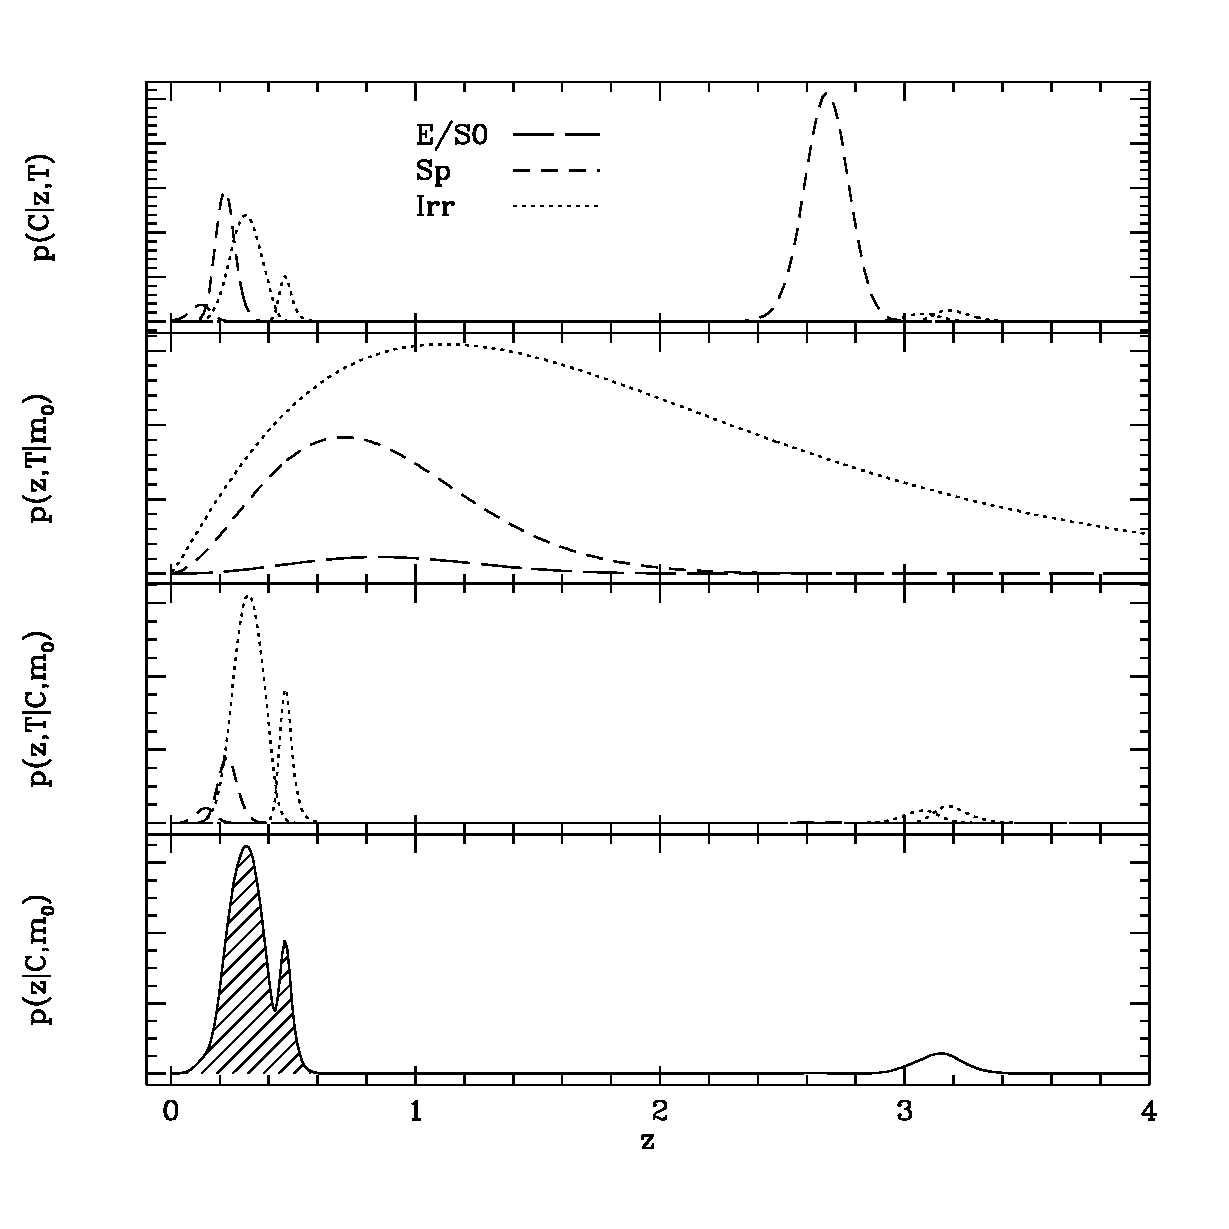
\includegraphics[width=1.3\textwidth]{figures/figpeaks.eps}
\end{adjustwidth*}
\caption{From \cite{Benitez.2000a}. This is a figure, simple and poorly drawn by my computer. The lines, intended to be physical representations of the glittering abstraction of pure length, have come out wobbly, like a plum pudding with too much plum. I will send my computer back to arithmetic class.}
\label{fig:myfig}
\end{figure}

\section{From redshift PDFs to stellar properties PDFs}
\label{sec:fit}

Given the PDF of the 

\section{Validation of the SED fitting}

In this section we show some results of simulations to determine how precise one can infer galaxies properties for a given set of magnitudes within the chosen filter set and 

\section{$V_{MAX}$ PDF}
\label{sec:vmax}



\chapter{Conclusions and Further work}


\bibliography{references}

%  Natbib citation types...
%    \citet{key}              ==>>  Jones et al. (1990)
%    \citep{key}              ==>>  (Jones et al. 1990)
%    \citep{key1,key2,...}    ==>>  (Jones et al. 1990; Smith 1989; ...)
%                                or (Jones et al. 1990, 1991; ...)
%                                or (Jones et al. 1990a,b; ...)
%    \citep*{key}             ==>>  (Jones, Baker, & Williams 1990)
%    \citep[chap. 2]{key}     ==>>  (Jones et al., 1990, chap. 2)
%    \citep[e.g.][]{key}      ==>>  (e.g. Jones et al., 1990)
%    \citep[see][p. 34]{key}  ==>>  (see Jones et al., 1990, p. 34)
%    \citealt{key}            ==>>  Jones et al., 1990
%    \citealt*{key}           ==>>  Jones, Baker, & Williams, 1990
%    \citealp{key}            ==>>  Jones et al. 1990
%    \citealp*{key}           ==>>  Jones, Baker, & Williams 1990
%    \citeauthor{key}         ==>>  Jones et al.
%    \citeauthor*{key}        ==>>  Jones, Baker, & Williams
%    \citeyear{key}           ==>>  1990
%    \citeyearpar{key}        ==>>  (1990)
%    \citetext{priv. comm.}   ==>>  (priv. comm.)


\end{document}